%%%%%%%%%%%%%%%%%%%%%%%%%%%%%%%%%%%%%%%%%%%%%%%%%%%%%%%%%%%%
%%  This Beamer template was created by Cameron Bracken.
%%  Anyone can freely use or modify it for any purpose
%%  without attribution.
%%
%%  Last Modified: January 9, 2009
%%

\documentclass[xcolor=x11names,compress]{beamer}

%% General document %%%%%%%%%%%%%%%%%%%%%%%%%%%%%%%%%%
\usepackage{graphicx}
\usepackage{tikz}
\usetikzlibrary{decorations.fractals}
%%%%%%%%%%%%%%%%%%%%%%%%%%%%%%%%%%%%%%%%%%%%%%%%%%%%%%


%% Beamer Layout %%%%%%%%%%%%%%%%%%%%%%%%%%%%%%%%%%
\useoutertheme[subsection=false,shadow]{miniframes}
\useinnertheme{default}
\usefonttheme{serif}
\usepackage{palatino}
\usepackage[english]{babel}
\usepackage{graphicx}

\setbeamerfont{title like}{shape=\scshape}
\setbeamerfont{frametitle}{shape=\scshape}

\setbeamercolor*{lower separation line head}{bg=DeepSkyBlue4} 
\setbeamercolor*{normal text}{fg=black,bg=white} 
\setbeamercolor*{alerted text}{fg=red} 
\setbeamercolor*{example text}{fg=black} 
\setbeamercolor*{structure}{fg=black} 
 
\setbeamercolor*{palette tertiary}{fg=black,bg=black!10} 
\setbeamercolor*{palette quaternary}{fg=black,bg=black!10} 

\renewcommand{\(}{\begin{columns}}
\renewcommand{\)}{\end{columns}}
\newcommand{\<}[1]{\begin{column}{#1}}
\renewcommand{\>}{\end{column}}
%%%%%%%%%%%%%%%%%%%%%%%%%%%%%%%%%%%%%%%%%%%%%%%%%%




\begin{document}


%%%%%%%%%%%%%%%%%%%%%%%%%%%%%%%%%%%%%%%%%%%%%%%%%%%%%%
%%%%%%%%%%%%%%%%%%%%%%%%%%%%%%%%%%%%%%%%%%%%%%%%%%%%%%

\begin{frame}
\title{EVALUATION OF WEB SECURITY MECHANISMS
	USING VULNERABILITY ANALYSIS \& PATTERN
	MINING}
%\subtitle{SUBTITLE}
\author{
	BIMAL VARGHESE\\
	\vspace{.2cm}
	Guide : Ms. SIMI STEPHEN\\\vspace{.2cm}
	{\it FISAT MOOKKANNOOR}\\
	\vspace{.3cm}
}
\date{
%	\begin{tikzpicture}[decoration=Koch curve type 2] 
%		\draw[DeepSkyBlue4] decorate{ decorate{ decorate{ (0,0) -- (3,0) }}}; 
%	\end{tikzpicture}  
%	\\
	\vspace{.5cm}
	\today
}
\titlepage
\end{frame}

%%%%%%%%%%%%%%%%%%%%%%%%%%%%%%%%%%%%%%%%%%%%%%%%%%%%%%
%%%%%%%%%%%%%%%%%%%%%%%%%%%%%%%%%%%%%%%%%%%%%%%%%%%%%%
\begin{frame}{Outline}
\tableofcontents
\end{frame}

\section{\scshape Introduction}
\begin{frame}{Introduction}
	\begin{itemize}
		\item  Usage of Web Applications are common these days
		\newline
		\item Internet boom have made them more popular to common man.
		\newline
		\item Usage include Social Networking, Online Banking,Online Shopping, Emails etc.
		\newline
		\item Global accessibility of  Web Applications increases its risk.
					
	\end{itemize}
	
\end{frame}

%\subsection{Need for Web Application Security}
\begin{frame}{Need for Web Application Security}
	\begin{itemize}
		\item Primary Responsibility - Application developers 
		\begin{itemize}
			\item Need to have an understanding of magnitude and relevance of assets they handle.
			\newline
		\end{itemize}
		\item Common reasons why securing a
		web application becomes tricky
		\begin{enumerate}
			\item Numerous languages and frameworks
			\item Exposure to huge number of audience
			\item Developer inexperience.
			\item Need for remote access of Organizational resources. 
		\end{enumerate}
	\end{itemize}
\end{frame}

%\subsection{Securing the Web Applications}
\begin{frame}{Securing the Web Applications}
	\begin{itemize}
		\item Security Standers
		\newline
		\item Tools for evaluating security.
		\newline
		\item Counter measures.
		\newline
		\item Proper Training.
		\newline
		\item Auditing and Patching 
	\end{itemize}
\end{frame}

%%%%%%%%%%%%%%%%%%%%%%%%%%%%%%%%%%%%%%%%%%%%%%%%%%%%%%
%%%%%%%%%%%%%%%%%%%%%%%%%%%%%%%%%%%%%%%%%%%%%%%%%%%%%%


\section{\scshape LITERATURE SURVEY}
%\subsection{frame 1}
\begin{frame}
\centering{\large{ \textbf{LITERATURE SURVEY}}}
\end{frame}
\begin{frame}{[1] Fault Injection and
		Dependability Evaluation of Fault-Tolerant Systems}
\begin{itemize}
\item Fault Injection in Traditional System.
\newline
\item Utilizes fault injection to explicitly remove design or implementation faults in a complex fault tolerant system.
\newline
\item Aims in reducing, by verification, the presence of faults
\newline
\item Faults injected to uncover potential issues and to improve the system
\end{itemize}
\end{frame}


\begin{frame}{[2] Xception: Software Fault Injection and Monitoring in Processor Functional Units}
	\begin{itemize}
		\item Software implemented fault injection (SWIFI) - for high complex systems.
		\newline
		\begin{itemize}
			\item Difficult to control and observe the fault effects
			inside the processor.
		
			\item Detection of the activated faults is very complex
			\newline
		\end{itemize}
		\item Simulation based fault injection is proposed.
		\newline
		\item Fault Emulation
		\begin{itemize}
			\item Application execution is interrupted
			\item Specific fault
			injection software code is executed.
		\end{itemize}
	\end{itemize}
\end{frame}

\begin{frame}{ [3] Emulation of Software Faults: A Field Data Study and	a Practical Approach}
	\begin{itemize}
		\item Injection of representative software faults.
		\newline
		\item Base principle - ``Software faults is the root cause of computer failures''.
		\newline
		\item Bugs in complex software have serious effect on the system.
		
	\end{itemize}
\end{frame}
\begin{frame}{Contd \dots}
	Software
	fault are injected according to following principle:
	
	\begin{itemize}
		\item Fault is injected to a component to evaluate the component in the presence of faulty component.
		
		\begin{itemize}
			\item Separation between target component and system under observation.
			
		\end{itemize}
		\item System behavior in presence of faulty component is observed.\newline
	\end{itemize}
	
	\begin{block}{Advantages.}
	\begin{enumerate}
		\item Validation of fault-tolerant mechanisms.
		\item  Prediction of worst-case scenarios and experimental risk assessment.
		\item  Dependability benchmarking.
	\end{enumerate}
	\end{block}
\end{frame}

\begin{frame}{[4] Using Attack Injection
		to Discover New Vulnerabilities}
	\begin{itemize}
		\item Existence
		of a vulnerability may not cause a security hazard until it is exploited.
		\item Intrusion can be prevented by removing vulnerability.
		\item Can be done at -
		\begin{enumerate}
			\item Development phase : identify programming flaws. 
			\item Operational phases : discovery of configuration errors and other similar problems.
		\end{enumerate} 
	\end{itemize}
\end{frame}
\begin{frame}{Contd \dots}

	\begin{itemize}

		\item  AJECT (Attack inJECtion Tool) used for
		vulnerability detection and removal.
		\newline
		\begin{enumerate}
			\item Simulates the behavior of an adversary by injecting attacks against a target system.
			\newline
			\item  Observes execution of the system to determine
			if the attacks have caused a failure.
			\newline
			\item If failure occur, presence of vulnerability identified and traditional debugging methods employed to fix it.
			\newline
		\end{enumerate}
		\item Experiment conducted with IMAP servers.
	\end{itemize}
\end{frame}
\begin{frame}{[5] Finding Security Vulnerabilities in Java Applications with
		Static Analysis}
	\begin{itemize}
		\item Popularity of Web Applications \& hidden Vulnerability in it.
		\item Exposure to wider audience.
		\item Inability of detection using firewalls \& other methods
		\begin{itemize}
			\item Attacks utilizes \textit{http} which is unhindered in firewalls.
		\end{itemize}
		\item High level languages (eg.Java) provides language level security.
		\begin{itemize}
			\item Restrict direct memory access.
			\item Automatic Garbage collection etc.
		\end{itemize}
		\item Logic errors can compromise Web Application security.
		\item Static code analysis detects these issues. 
	\end{itemize}
\end{frame}

\begin{frame}{[6] An Empirical Analysis of Input Validation Mechanisms}
	\begin{itemize}
		\item Application Security \& Programing Language efficiency.
		\newline
		\begin{itemize}
			\item How bad a programing languages in term of propensity of mistakes.\newline
		\end{itemize}
		\item Type System (Strong / Weak) \& Type checking (Static / Dynamic) in software robustness.
		\newline
		\item A strong typed language with a
		static type checking can help deliver a safer application without affecting its performance
	\end{itemize}
\end{frame}

\begin{frame}{[7] Preliminary Results
		on Using Static Analysis Tools for Software Inspection.}
	\begin{itemize}
		\item Software code inspections \& Software Quality
		\begin{itemize}
			\item Can detect as little
			as 20\% to as much as 93\% of number of defects in a software.\newline
		\end{itemize}
		\item Defect classification scheme was proposed.\newline
		\item Vulnerability
		discovery’s model(VDM)
		\begin{itemize}
			\item Ability of a system to perform
			its required functions without software-caused violations of its explicit or implicit security
			policy.
			
		\end{itemize}
	
	\end{itemize}
\end{frame}
\begin{frame}{Contd \dots}
	Two nature of software systems are considered.
	\newline
		\begin{enumerate}
			\item Engineering nature:
			\begin{itemize}
				\item Employs statistical analysis of vulnerabilities
				\item  Features like when was a vulnerability introduced, when was it discovered, how is the source code of a system changing, etc.
				
			\end{itemize}
			\item Economic nature:
			\begin{itemize}
				\item Features like what is the auction-ascertained price of a previously-unreported vulnerability in a specific system.
				\item First person to report vulnerability receives the reward.
			\end{itemize}
		\end{enumerate} 

\end{frame}

\begin{frame}{[8] Semi-Automatic Security Testing of Web
		Applications from a Secure Model}
	\begin{itemize}
		\item Non Monolithic nature and Distributed components in Web Applications.\newline
		\item White-box penetration testing:
		\begin{itemize}
			\item All applications are to develop in the same language
			\newline
		\end{itemize}
		\item Black-box penetration testing:
		\begin{itemize}
			\item Not highly effective because of weaknesses of the crawling step which misses lots
			of potential interaction with the user
		\end{itemize}
		\item Model checkers for security analysis
		was proposed
	\end{itemize}
\end{frame}
\begin{frame}{Contd \dots}
	\begin{itemize}
		\item For System Under Validation
		(SUV),formal model \textbf{M} is used.
		\item Vulnerability is injected by mutating the formal model of the web application.
		\item Model checker outputs attack traces that exploit those vulnerabilities.
		\item Attack traces are translated into concrete test cases.
		\item Tests are executed on the real system using an automatic procedure
	\end{itemize}
\end{frame}

\begin{frame}{[9] Gauging Software Readiness with De-
		fect Tracking}
\begin{itemize}
	\item In competitive commercial market,time of release is very important for software.
	\item Strict Deadlines have to be met for programmers.
	\item Softwares with known bugs are released to meet the time.
	\newline
	\item To judge, if a software is ready to meet the market  
	\begin{itemize}
		\item Measure defect density ie, number of defects per line of code
		\item Separate defect reports into groups and track them separately
	\end{itemize}
\end{itemize}
\end{frame}
\begin{frame}{contd \dots}
	\begin{itemize}
		\item Track the number of defects reported in each pool and the number of total
		defects reported. \newline
		{ $ Defects_{total} = \frac{Defects_{ A} * Defects_{ B}}{Defects_{ (A+B)}} $}\newline
		\item The number of unique defects reported at any given time is: \newline
		 $ Defects_{ unique} = Defects _{A} +  Defects_{ B} - Defects_{ (A+B)} $
	\end{itemize}
	where A \& B two groups considered
\end{frame}
%\subsection{METHODS COMPARISON}
\begin{table}[H]
	\begin{center}
		\small
		\caption{Comparison of various vulnerability analysis methods}
		\scalebox{0.8}{
		\begin{tabular}{|p{.95cm} | p{5cm} | p{2.5cm}| p{2.75cm} | }%  {|c|c|c|}
			\hline\textbf{Sl.No.} & \qquad \qquad \textbf{Paper Name}  & \textbf{Method Used} & \textbf{Implemented on} \\ 
			\hline 1 & Fault Injection and
			Dependability Evaluation of Fault-Tolerant Systems  & Fault Injection  & Hardware Level \\ 
			\hline 2 & Xception: Software Fault Injection and Monitoring in Processor Functional Units & Fault Injection & Software Simulation \\ 
			\hline 3 & Emulation of Software Faults:
			A Field Data Study and a Practical Approach & Bug Injection & Software Components \\ 
			\hline 4 & Using Attack Injection to Discover 
			New Vulnerabilities  & Server Software & IMAP \\ 
			\hline 5 & Finding Security Vulnerabilities in Java Applications with	Static Analysis & Static Code Analysis & Java \\ 
			\hline 6 & Preliminary Results on Using Static Analysis Tools for Software Inspection  & Source Code Analysis & Coding Standard \\ 
			\hline 7 & Semi-Automatic Security Testing of  Web
			Applications from a Secure Model  & Modal Analysis & Web Application Model \\ 
			\hline 8 &
			Gauging Software Readiness with Defect Tracking
			& Defect Density & Software Defects\\
			\hline
			
		\end{tabular} 
	}
	\end{center}
\end{table}

%%%%%%%%%%%%%%%%%%%%%%%%%%%%%%%%%%%%%%%%%%%%%%%%%%%%%%
%%%%%%%%%%%%%%%%%%%%%%%%%%%%%%%%%%%%%%%%%%%%%%%%%%%%%%


%%%%%%%%%%%%%%%%%%%%%%%%%%%%%%%%%%%%%%%%%%%%%%%%%%%%%%
%%%%%%%%%%%%%%%%%%%%%%%%%%%%%%%%%%%%%%%%%%%%%%%%%%%%%%
\section{\scshape METHODOLOGY}
%\subsection{frame 1}
\begin{frame}
	\centering{\large{ \textbf{METHODOLOGY}}}
\end{frame}
\begin{frame}{METHODOLOGY}
\begin{itemize}
	\item Based on injection of realistic vulnerabilities and the
	subsequent controlled exploit of those vulnerabilities to attack the system.
	\newline
	\item Can be  used to test counter measure mechanisms\\
	Like IDS, Firewalls etc.
	\newline
	\item Vulnerability Attack Injection tool (VAIT) is created.
	\newline
	\item Inspects application for input validation vulnerabilities.\\
	Like SQLi,XSS etc.
\end{itemize}
\end{frame}
\begin{frame}

\begin{figure}
\centering
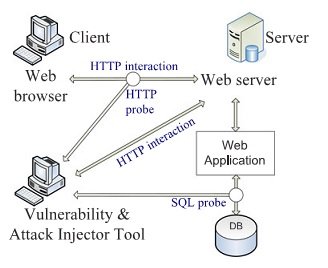
\includegraphics[width=0.7\linewidth]{Main/Fig2}
\caption{VAIT setup}
\label{fig:Fig2}
\end{figure}

\end{frame}

%%%%%%%%%%%%%%%%%%%%%%%%%%%%%%%%%%%%%%%%%%%%%%%%%%%%%%
%%%%%%%%%%%%%%%%%%%%%%%%%%%%%%%%%%%%%%%%%%%%%%%%%%%%%%
%\subsection{ATTACK PROCEDURE}
\begin{frame}{ATTACK PROCEDURE}
	4 main stages \newline
\begin{enumerate}
	\item Preparation stage
	\begin{itemize}
		\item Crawls Web Application.
		\item Analyze HTTP \& SQL communications.
		\item Generate correlation between http input and SQL queries
	\end{itemize}
	\item  Vulnerability injection stage
	\begin{itemize}
		\item Analyze source code.
		\item Inject vulnerability.
		\begin{itemize}
			\item Done by removing
			the protection of the target variables \\say call to a sanitizing function
		\end{itemize}
		\item perform specific code mutation in order to inject one vulnerability in that particular location.
	\end{itemize}
	
\end{enumerate}
\end{frame}

\begin{frame}{Contd \dots}
	\begin{enumerate}
			\item [3] Attackload generation stage
			\begin{itemize}
				\item Attackload - Malicious activity data, needed to attack a given vulnerability
				\item Built around the interaction patterns derived from the preparation stage
				\begin{itemize}
					\item Through fuzzing process. 
					\item prefix $ (>,),`,``, \dots) $
					\item suffix $ (<,–,\#,`,",\dots) $
				\end{itemize}
			
			\end{itemize}
			\item [4] Attack stage
			\begin{itemize}
				\item  Malicious interaction with web application.
				\item Alter SQL query or HTML data.
				\item Vulnerable source code files are injected one at a time.
				\item SQL \& HTTP probes are again deployed.
				\item Attack footprints analyzed for success.
			\end{itemize}
	\end{enumerate}
\end{frame}
%\subsection{VULNERABILITY \& ATTACK INJECTOR
%	TOOL}
\begin{frame}{VULNERABILITY \& ATTACK INJECTOR
		TOOL}
	\begin{itemize}
		\item VAIT - performs attack injection methodology.\newline
		\item Targets Linux,Apache. MySQL, PHP (LAMP) applications.\newline
		\item Process done with minimum human intervention.\newline
		\item Interactions can be manual or through automating tools.\newline
		\item Monitoring done using built in proxies. 
	\end{itemize}
\end{frame}
%%%%%%%%%%%%%%%%%%%%%%%%%%%%%%%%%%%%%%%%%%%%%%%%%%%%%%
%%%%%%%%%%%%%%%%%%%%%%%%%%%%%%%%%%%%%%%%%%%%%%%%%%%%%%
%\subsection{VAIT architecture}
\begin{frame}{VAIT architecture.}
\begin{figure}
\centering
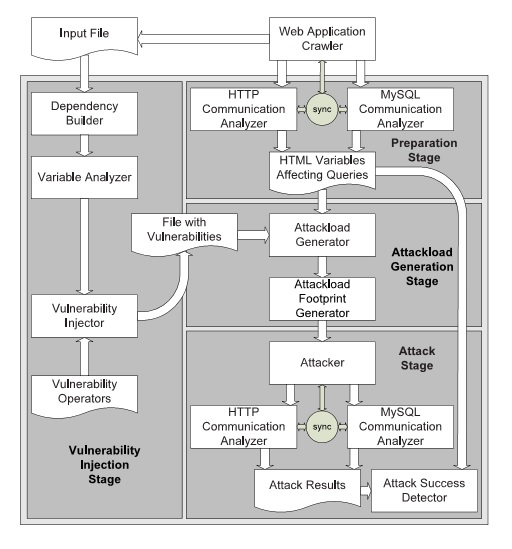
\includegraphics[width=0.7\linewidth]{Main/fig7}
\caption{VAIT architecture.}
\label{fig:fig7}
\end{figure}

\end{frame}
\begin{frame}
	\begin{itemize}
		\item SQLi \& XSS attacks web Application.\newline
		\item Remote Code Execution (RCE) \& File Inclusion (FI) attacks the system on which the application runs.\newline
		\item VAIT tool will be modified so as to identify other validation errors like RCE \& FI.\newline
		\item By utilizing Pattern mining methods, VAIT tool can identify similar vulnerability of web applications .
	\end{itemize}
\end{frame}

\section{CONCLUSION}
\begin{frame}
	\centering{\large{ \textbf{CONCLUSION}}}
\end{frame}
\begin{frame}{CONCLUSION}
	\begin{itemize}
		\item Methodology can analyze, validation vulnerabilities in Web Applications \newline
		\item Vulnerabilities are derived from extensive field study.\newline
		\item VAIT tool will be able to identify validation issues.\newline
		\item VAIT tool can be modified to identify similar vulnerability of web applications .
	\end{itemize}
\end{frame}
\section*{REFERRENCES}
\begin{frame}
	\centering{ \huge \textbf{REFERRENCES}}
\end{frame}


\begin{frame}[allowframebreaks]{REFERRENCES}
	\tiny
\setbeamertemplate{bibliography item}{\insertbiblabel}
\begin{thebibliography}{8}
%	\addcontentsline{toc}{chapter}{\bf BIBLIOGRAPHY}
	
	\bibitem{1}
	cgisecurity.net, www.cgisecurity.com/articles/csrf-faq.shtml\#
	whatis, Dec. 2008.
	
	\bibitem{2}
	G. Alvarez and S. Petrovic,  ``A New Taxonomy of Web Attacks Suitable for Efficient Encoding,'' Computers and Security, vol. 22,
	no. 5, pp. 435-449, July 2003
	
	
	
	\bibitem{3}
	S. Christey and R. Martin,  ``Vulnerability Type Distributions in
	CVE,'' Mitre Report, May 2007.
	
	\bibitem{4}
	J. Duraes and H. Madeira,  ``Emulation of Software Faults: A Field
	Data Study and a Practical Approach,'' IEEE Trans. Software Eng.,
	vol. 32, no. 11, pp. 849-867, Nov. 2006.
	
	\bibitem{5}
	M.R. Lyu, Handbook of Software Reliability Engineering. IEEE
	Computer Society Press \& McGraw-Hill, 1996.
	
	\bibitem{6}
	J. Williams and D. Wichers,  ``OWASP Top 10,'' OWASP Foundation, Feb. 2013.
	
	\bibitem{7}
	N. Neves, J. Antunes, M. Correia, P. Verissimo, and R. Neves,
	``Using Attack Injection to Discover New Vulnerabilities,'' Proc.
	IEEE/IFIP Int’l Conf. Dependable Systems and Networks, 2006.
	
	\bibitem{8}
	J. Fonseca, M. Vieira, and H. Madeira,  ``Testing and Comparing
	Web Vulnerability Scanning Tools for SQLi and XSS Attacks,''
	Proc. IEEE Pacific Rim Int’l Symp. Dependable Computing, Dec. 2007.
	
	\bibitem{9}
	S. Clowes,  ``A Study in Scarlet, Exploiting Common Vulnerabilities in PHP Applications,'' http://www.securereality.com.au/
	studyinscarlet.txt, 2013.
	
	\bibitem{10}
	B. Livshits and S. Lam,  ``Finding Security Vulnerabilities in Java
	Applications with Static Analysis,'' Proc. USENIX Security Symp.,
	pp. 18-18, 2005.
	
	\bibitem{11}
	M. Buchler, J. Oudinet, and A. Pretschner,  ``Semi-Automatic Security Testing of Web Applications from a Secure Model,'' Proc. Int’l
	Conf. Software Security and Reliability, 2012.
	
	\bibitem{12}
	S. McConnell, ``Gauging Software Readiness with Defect
	Tracking'', IEEE Software, vol. 14, no. 3, May/June 1997.
	
	\bibitem{13}
	N. Nagappan, L. Williams, J. Hudepohl, W. Snipes, M. Vouk,
	``Preliminary Results on Using Static Analysis Tools for Software
	Inspection.'' Proc. Int’l Symp. Software Reliability Eng., pp. 429-439,
	2004.
	\bibitem{14}
	OSVDB,  ``Open Sourced Vulnerability Database,'' http://osvdb.
	org, May 2013.
	\bibitem{15}
	D. Powell and R. Stroud,  ``Conceptual Model and Architecture of
	MAFTIA,'' Project MAFTIA, Deliverable D21, 2003.
	
	\bibitem{16}
	J. Fonseca and M. Vieira,  ``Mapping Software Faults with Web
	Security Vulnerabilities,'' Proc. IEEE/IFIP Int’l. Conf. Dependable
	Systems and Networks, June 2008
	
	\bibitem{17}
	S. Fogie, J. Grossman, R. Hansen, A. Rager, and P. Pektov, XSS
	Attacks: Cross Site Scripting Exploits and Defense. Syngress, 2007.
	Intell., vol. 32, no. 6, pp. 1127–1133, Jun. 2010.
	\bibitem{18}
	J. Arlat, A. Costes, Y. Crouzet, J.-C. Laprie, and D. Powell,  ``Fault
	Injection and Dependability Evaluation of Fault-Tolerant Systems,'' IEEE Trans. Computers, vol. 42, no. 8, pp. 913-923, Aug.
	1993.
	\bibitem{19}
	T. Scholte et al.,  ``An Empirical Analysis of Input Validation
	Mechanisms,'' Proc. ACM Symp. Applied Computing, pp. 1419-1426,
	2012.
	
	\bibitem{20}
	J. Carreira, H. Madeira, and J.G. Silva,  ``Xception: Software Fault
	Injection and Monitoring in Processor Functional Units,'' IEEE
	Trans. Software Eng., vol. 24, no. 2, Feb. 1998.
	
	\bibitem{21}
	N. Tomatis, R. Brega, G. Rivera, and R. Siegwart,  ``May You Have
	a Strong (-Typed) Foundation’ Why Strong Typed Programming
	Languages Do Matter,'' Proc. IEEE Int’l Conf. Robotics and
	Automation, 2004.
	
	\bibitem{22}
	J. Christmansson and R. Chillarege,  ``Generation of an Error Set
	that Emulates Software Faults,'' Proc. IEEE Fault Tolerant Computing Symp., 1996.
	\bibitem{23}
	H Madeira, M. Vieira, and D. Costa,  ``On the Emulation of Software Faults by Software Fault Injection,'' Proc. IEEE/IFIP Int‘l
	Conf. Dependable System and Networks, 2000.
	
	\bibitem{24}
	M. Cukier, R. Berthier, S. Panjwani, and S. Tan,  ``A Statistical
	Analysis of Attack Data to Separate Attacks,'' Proc. Int’l Conf.
	Dependable Systems and Networks, pp. 383-392, 2006.
	
\end{thebibliography}
\end{frame}
\begin{frame}
	\centering{ \huge \textbf{THANK YOU}}
\end{frame}


\end{document}